\documentclass[tikz,border=8pt]{standalone}
\usepackage{amsmath}
\usetikzlibrary{arrows.meta,patterns}
\begin{document}
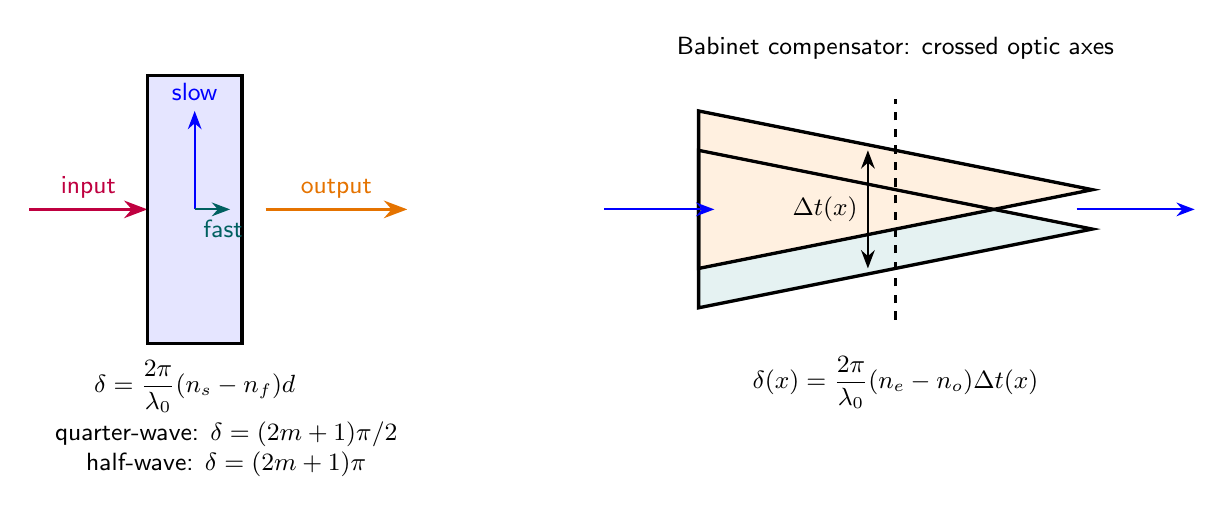
\begin{tikzpicture}[font=\sffamily\small,>=Stealth,thick]
  \begin{scope}
    \draw[->,purple,very thick] (-1.5,0)--(0,0) node[midway,above] {input};
    \fill[blue!10] (0,-1.7) rectangle (1.2,1.7);
    \draw[very thick] (0,-1.7) rectangle (1.2,1.7);
    \draw[->,blue] (.6,0)--(.6,1.25) node[above] {slow};
    \draw[->,teal!75!black] (.6,0)--(1.05,0) node[pos=.8,below] {fast};
    \draw[->,orange!90!black,very thick] (1.5,0)--(3.3,0) node[midway,above] {output};
    \node[align=center] at (.6,-2.25)
      {$\displaystyle \delta=\frac{2\pi}{\lambda_0}(n_s-n_f)d$};
    \node[align=center] at (1,-3.05)
      {quarter-wave: $\delta=(2m+1)\pi/2$\\half-wave: $\delta=(2m+1)\pi$};
  \end{scope}
  \begin{scope}[xshift=7cm]
    \fill[teal!10] (0,-1.25)--(5,-.25)--(0,.75)--cycle;
    \fill[orange!12] (0,1.25)--(5,.25)--(0,-.75)--cycle;
    \draw[very thick] (0,-1.25)--(5,-.25)--(0,.75)--cycle;
    \draw[very thick] (0,1.25)--(5,.25)--(0,-.75)--cycle;
    \draw[->,blue] (-1.2,0)--(.2,0);
    \draw[->,blue] (4.8,0)--(6.3,0);
    \draw[dashed] (2.5,-1.4)--(2.5,1.4);
    \draw[<->] (2.15,-.75)--(2.15,.75) node[midway,left] {$\Delta t(x)$};
    \node at (2.5,2.05) {Babinet compensator: crossed optic axes};
    \node[align=center] at (2.5,-2.2)
      {$\displaystyle \delta(x)=\frac{2\pi}{\lambda_0}(n_e-n_o)\Delta t(x)$};
  \end{scope}
\end{tikzpicture}
\end{document}
